%%%%%%%%%%%%%%%%%%%%%%%%%%%%%%%%%%%%%%%%%
% Journal Article
% LaTeX Template
% Version 2.0 (February 7, 2023)
%
% This template originates from:
% https://www.LaTeXTemplates.com
%
% Author:
% Vel (vel@latextemplates.com)
%
% License:
% CC BY-NC-SA 4.0 (https://creativecommons.org/licenses/by-nc-sa/4.0/)
%
% NOTE: The bibliography needs to be compiled using the biber engine.
%
%%%%%%%%%%%%%%%%%%%%%%%%%%%%%%%%%%%%%%%%%

%----------------------------------------------------------------------------------------
%	PACKAGES AND OTHER DOCUMENT CONFIGURATIONS
%----------------------------------------------------------------------------------------

\documentclass[
	a4paper, % Paper size, use either a4paper or letterpaper
	10pt, % Default font size, can also use 11pt or 12pt, although this is not recommended
	unnumberedsections, % Comment to enable section numbering
	twoside, % Two side traditional mode where headers and footers change between odd and even pages, comment this option to make them fixed
]{LTJournalArticle}

\usepackage{float}
\usepackage{hyperref}
\usepackage{parskip}
\usepackage{pgfplots}
\usepackage{csvsimple}
\usepackage{booktabs}
\usepackage[utf8]{inputenc}


\addbibresource{sample.bib} % BibLaTeX bibliography file

\runninghead{} % A shortened article title to appear in the running head, leave this command empty for no running head

\footertext{\textit{Computer graphics course paper} (2023) Beijing Jiaotong University, School of Software} % Text to appear in the footer, leave this command empty for no footer text

\setcounter{page}{1} % The page number of the first page, set this to a higher number if the article is to be part of an issue or larger work

%----------------------------------------------------------------------------------------
%	TITLE SECTION
%----------------------------------------------------------------------------------------

\title{Exploring Block-Based\\ Traversal Sampling Algorithms\\  in Polygon Rasterization} % Article title, use manual lines breaks (\\) to beautify the layout

% Authors are listed in a comma-separated list with superscript numbers indicating affiliations
% \thanks{} is used for any text that should be placed in a footnote on the first page, such as the corresponding author's email, journal acceptance dates, a copyright/license notice, keywords, etc
\author{%
	Sichao He\textsuperscript{1}
}

% Affiliations are output in the \date{} command
\date{\footnotesize\textsuperscript{\textbf{1}}School of Software, Beijing Jiaotong University}

% Full-width abstract
\renewcommand{\maketitlehookd}{%
	\begin{abstract}\vspace{10pt}
		Rasterization is a critical process in the field of computer graphics, transforming vector descriptions into a raster format. Traditional methods often involve evaluating each individual pixel within a bounding box to determine whether it lies inside the target shape or optimizing it by using traversal algorithm. However, this approach can lead to performance losses due to the unnecessary computation of non-overlapping regions. To address this issue, this paper presents an innovative Block-Based Traversal Sampling algorithm for rasterization. This technique divides the bounding box into multiple blocks, calculating overlaps  between each block and the target 2D polygon according to Separating Axis Theorem. Only the overlapping blocks are evaluated by traversal algorithm then sampled, effectively omitting the computation for non-overlapping regions. The algorithm in this paper combines the advantages of these two methods and is further optimized by a method similar to Block Sparse algorithm. By this means, the proposed method significantly reduces computational overhead and enhances performance, thereby offering a promising alternative for efficient rasterization in computer graphics.	\end{abstract}
}

%----------------------------------------------------------------------------------------

\begin{document}

\maketitle % Output the title section

%----------------------------------------------------------------------------------------
%	ARTICLE CONTENTS
%----------------------------------------------------------------------------------------

\section{Introduction}

The rapid rendering of 3D Z-buffered, linearly interpolated polygons is a foundational problem in computer graphics. This problem is generally comprised of two components: 1) the three-dimensional transformation, projection, and illumination computations of the vertices, and 2) the rasterization of the polygon onto a frame buffer. This paper specifically addresses one facet of the second component, namely, the computation of the polygon's boundaries.


\subsection{Cross-product Operation}
\begin{figure}[H] % Single column figure
	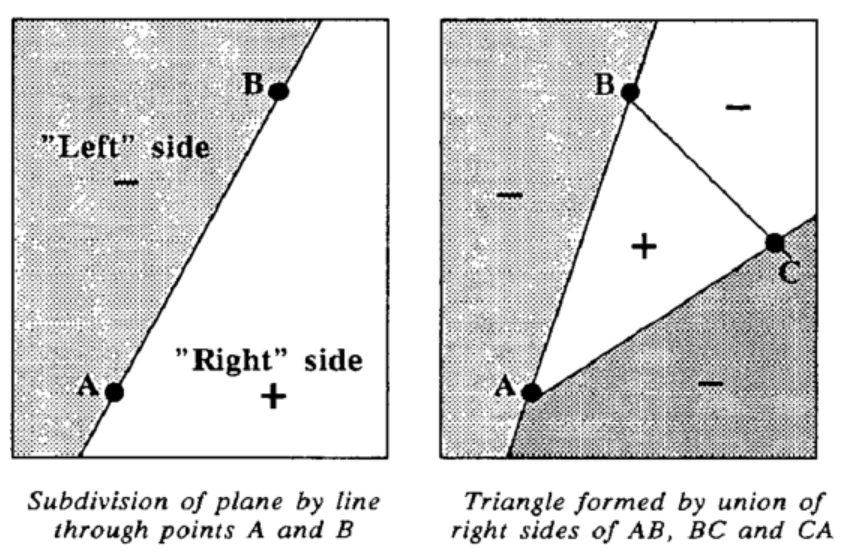
\includegraphics[width=\linewidth]{1.png}
	\caption{A Triangle Can be Formed by Combination of Edges}
\end{figure}

Figure 1 shows how it is possible to define a triangle by the union of three edges which are specified by edge functions. It is possible to define more complex polygons by using boolean combinations of more than three edges.
Traditionally, each pixel is considered a point to evaluate its positional relation with the polygon. This is achieved by conducting a cross-product operation on the edges of the polygon, which results in determining the sides of each edge the point lies on. This eventually helps us understand whether a pixel resides within a triangle.\cite{pineda1988}

\subsection{Bounding Box Algorithm}

Naturally, enhancing the performance of this algorithm during the rasterization sampling phase is crucial, especially given the significant overhead required to determine the position of each pixel within the triangle. The first significant performance-enhancing strategy was the introduction of the bounding box algorithm.

\begin{figure}[H] % Single column figure
	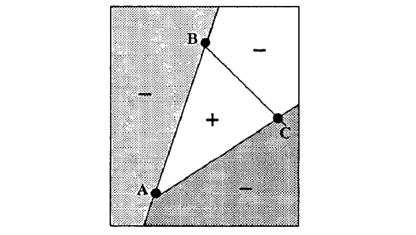
\includegraphics[width=\linewidth]{2.png}
	\caption{Bounding Box Algorithm diagram}
\end{figure}

Figure2 shows the bounding box algorithm, simply put, is a method that encapsulates a polygon within a rectangle that is large enough to contain it.\cite{yunhong1999} By creating a bounding box, unnecessary computations are reduced, as it eliminates the need to perform calculations for pixels outside the box. This results in significant performance savings by localizing the bounding box alone.

\subsection{Traversal Algorithm}

Further optimization was achieved through revising the order of traversal, with the development of the Traversal Algorithm. This algorithm ensures the coverage of all pixels in a polygon. Figure 3 illustrates two basic algorithms. The simplest strategy is to traverse the bounding box; however, it is not typically the most efficient. A more intelligent algorithm would move to the next line once it goes beyond the edge of a triangle.

\begin{figure}[H] % Single column figure
	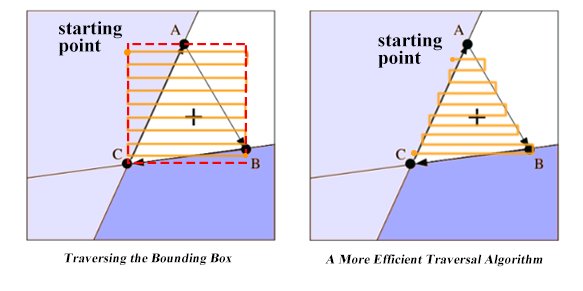
\includegraphics[width=\linewidth]{3.png}
	\caption{Simple Traversal Algorithms}
\end{figure}

A significant complication of this intelligent algorithm is that when it advances to the subsequent line, it might enter the triangle. In such instances, the algorithm must first seek the edge's exterior before initiating the next scan line.\cite{pineda1988} An example of this issue is demonstrated on the top right-hand edge of the triangle in Figure 4.

\begin{figure}[H] % Single column figure
	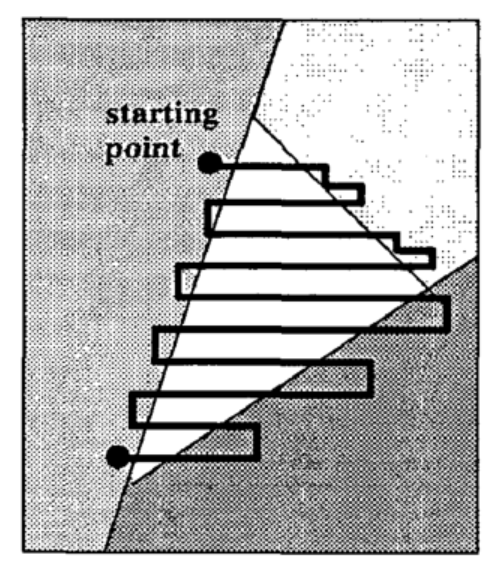
\includegraphics[width=\linewidth]{4.png}
	\caption{Traversal Algorithms May Have to Search for Edge}
\end{figure}

An even smarter algorithm is illustrated in Figure 5. This algorithm descends from the starting point, gradually expanding from a center line. This algorithm's advantage over the simpler one is that it never needs to seek an edge, then backtrack. However, the tradeoff is that the interpolator state for the center line must be preserved while traversing the outer points, since the interpolators must be re-initiated back at the center line. It should be noted that at the bottom, the "center" line shifts over if it ends up exterior to the triangle.

\begin{figure}[H] % Single column figure
	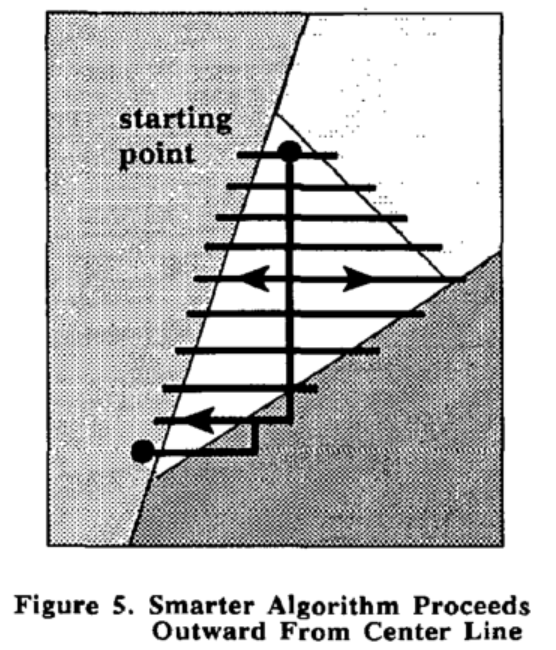
\includegraphics[width=\linewidth]{5.png}
	\caption{Smarter Algorithm Proceeds Outward From Center Line}
\end{figure}

\subsection{Block Sparse Algorithm}
Although the Traversal Algorithm also considers slicing for parallel optimization, it doesn't elaborate on how to select the corresponding slice. Thus, in this paper, the Block-Based Traversal Algorithm is introduced to optimize this process, following the example of OpenAI's Block Sparse Algorithm.

Figure 6 shows the basic thinking of Block Sparse Algorithm, it enhances computational efficiency by concentrating the computation on blocks of the input matrix with high magnitude. It divides the matrix into several blocks, then based on a certain threshold, only processes the blocks containing significant values while skipping over those with low magnitude.\cite{gray2017}

\begin{figure}[H] % Single column figure
	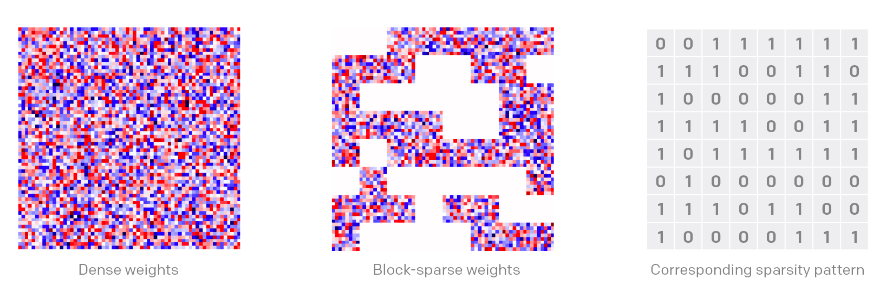
\includegraphics[width=\linewidth]{6.png}
	\caption{OpenAI: Block Sparse GPU kernels}
\end{figure}

Applying a similar concept, we calculate whether each block rectangle in the bounding box overlaps with the polygon to determine whether this block should be selected for Traversal Algorithm calculations. The overlap between two polygons can be determined by checking if any edge of each block rectangle intersects with any edge of the target polygon. If they intersect, then the block undeniably overlaps with the polygon.

Therefore, the flow of this algorithm involves determining the bounding box, dividing the bounding box according to the block size, and then generating a block mask Boolean matrix by judging whether each block overlaps using Separating Axis Theorem.\cite{gottschalk1996} Following this, the Traversal Algorithm is applied in parallel to each bounding box, producing the final sampling results.
%------------------------------------------------

\section{Block-based Traversal Implementation}

The source code for the implementation is available on GitHub at \href{https://github.com/Routhleck/Block-based-Traversal-algorithm}{this link}\footnote{https://github.com/Routhleck/Block-based-Traversal-algorithm}.
The Block-based Traversal method in this algorithm is implemented mainly in the function \texttt{rasterization\_traversal\_block}. Here, the key steps of the process are explained.

\subsection{Initialization}

First, a two-dimensional field (array) is initialized with boolean values, with size equivalent to the input field size (\texttt{field\_size}). All values are initially set to False (0).

\begin{verbatim}
field = np.zeros(field_size, dtype=np.bool_)
\end{verbatim}

\subsection{Bounding box generation}
Next, a list of bounding boxes is generated for all polygons in the input polygon list (\texttt{polygonList}) using the function \texttt{generateBoundingBoxes}. A bounding box is a smallest rectangular box which contains the polygon. The coordinates of the bounding box corners are determined by the minimum and maximum $x$ and $y$ values of the polygon vertices.

\subsection{Block Mask Generation}

For each polygon, a boolean mask of blocks is calculated, indicating which blocks the polygon intersects with. This is achieved by calling the function \texttt{calculateMaskFromPolygon}. For each block within the bounding box of the polygon, a rectangle is defined and its intersection with the polygon is checked using the function \texttt{isRectangleInPolygon}. The output of this function is a boolean value indicating whether there is an intersection or not.

\subsection{Field Traversal}

After generating the mask for a polygon, the field is traversed and modified based on the mask using the function \texttt{traverseMask}. For each block in the mask that is True (i.e., it intersects with the polygon), a more detailed traversal is conducted using the function \texttt{traverseBlock}. In this function, the algorithm searches for the start point within the block that is inside the polygon, and then it scans the block, marking the points within the polygon in the field. This is conducted by moving to the right until the edge of the polygon or the block is reached, and then moving down to the next row to repeat the process, until the entire block is scanned.

\subsection{Just-in-time Compilation}

To improve the performance of the algorithm and make the algorithm parallel, the NumPy and Numba libraries are used, specifically the functions decorated with \texttt{@jit} and \texttt{@njit}. This allows for just-in-time (JIT) compilation of the Python code to machine code, leading to much faster execution times.

%------------------------------------------------
\section{Methodologies}

\subsection{Test Introduction}

The functionality and performance of the rasterization methods were tested on three polygon lists of varying complexity, each with different field sizes. The polygon lists were defined as numpy arrays, each containing a number of 2D arrays, with each 2D array representing a polygon specified by its vertices. The field sizes ranged from 600 x 600 to 2400 x 2400.

Additionally, we evaluated the impact of varying the block size on the performance of the block-based traversal method. The block sizes considered ranged from 25 x 25 to 400 x 400.

For fairer testing, parallel processing is also performed for Traversal Algorithm, both of which are taking same block size for splitting blocks

\begin{figure}[H] % Single column figure
	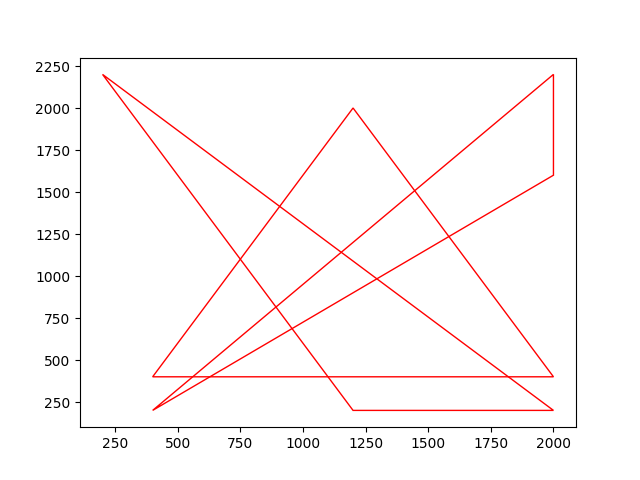
\includegraphics[width=\linewidth]{origin_triangle.png}
	\caption{Origin Triangle to be Rasterized}
\end{figure}

\begin{figure}[H] % Single column figure
	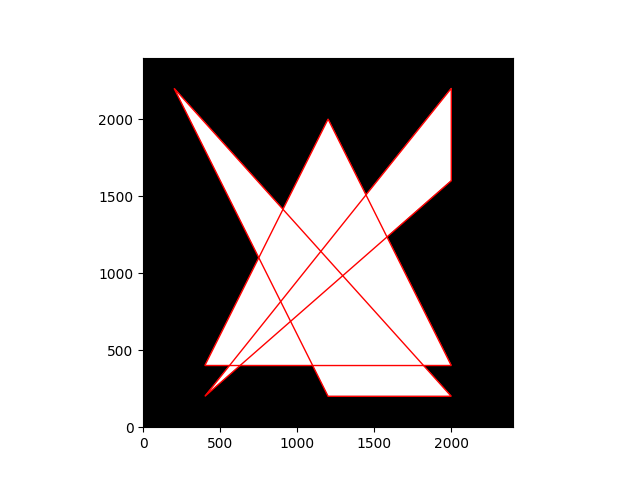
\includegraphics[width=\linewidth]{rasterization_triangle.png}
	\caption{The result of rasterization}
\end{figure}

Figure 7 shows the origin triangle to be rasterized. The field size is 2400 x 2400. And Figure 8 is the result of rasterization.

\subsection{Test Procedure}

The test procedure is as follows:

\begin{enumerate}
    \item Initialize the custom polygon list using the \texttt{initPolygonList\_custom} function.
    
    \item The block-based traversal method is run twice: the first time to warm up the JIT compiler, and the second time to measure the execution time. The output is a Boolean field indicating whether each pixel is inside a polygon, and the elapsed time.
    
    \item Similarly, the traversal method is run twice, also capturing the Boolean field and the elapsed time.
\end{enumerate}

This test process is repeated for each combination of polygon list, field size, and block size.

\section{Result}

From the experimental results shown in the table and graph, we can draw some conclusions about the performance of the two algorithms - the Parallel Traversal and Block-based Traversal.

\begin{figure}[H] % Single column figure
	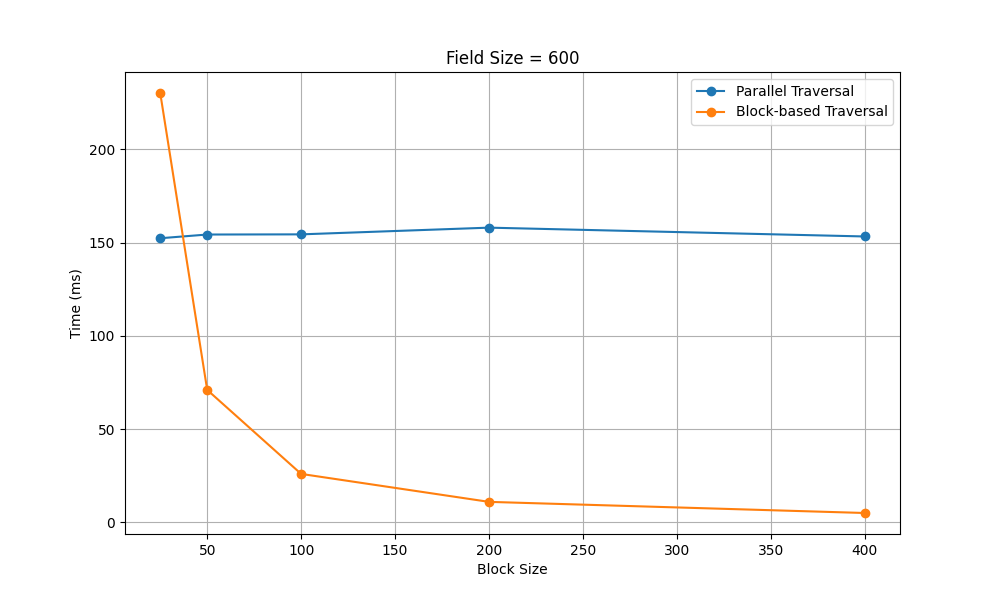
\includegraphics[width=\linewidth]{field_600.png}
	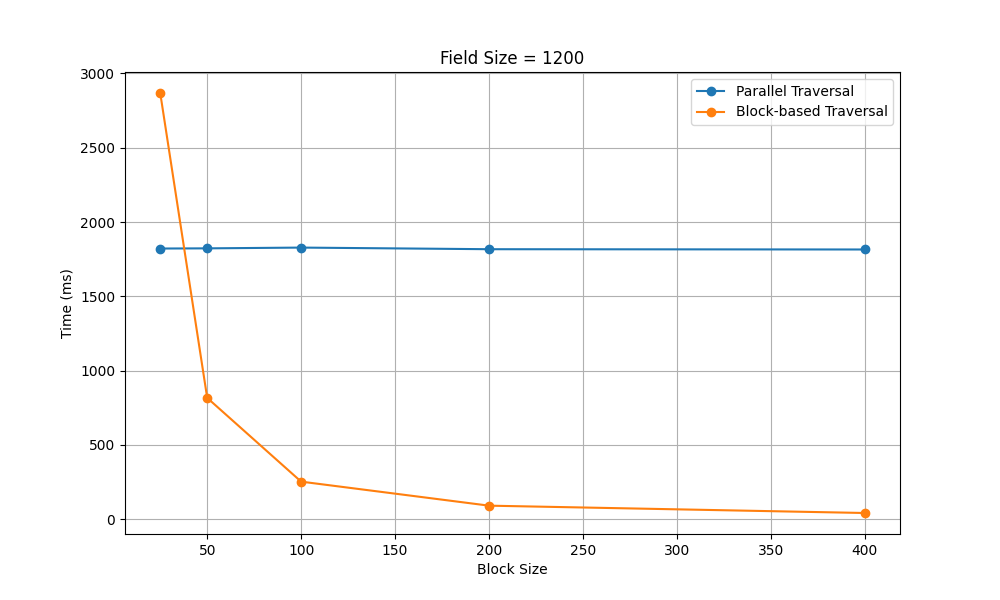
\includegraphics[width=\linewidth]{field_1200.png}
	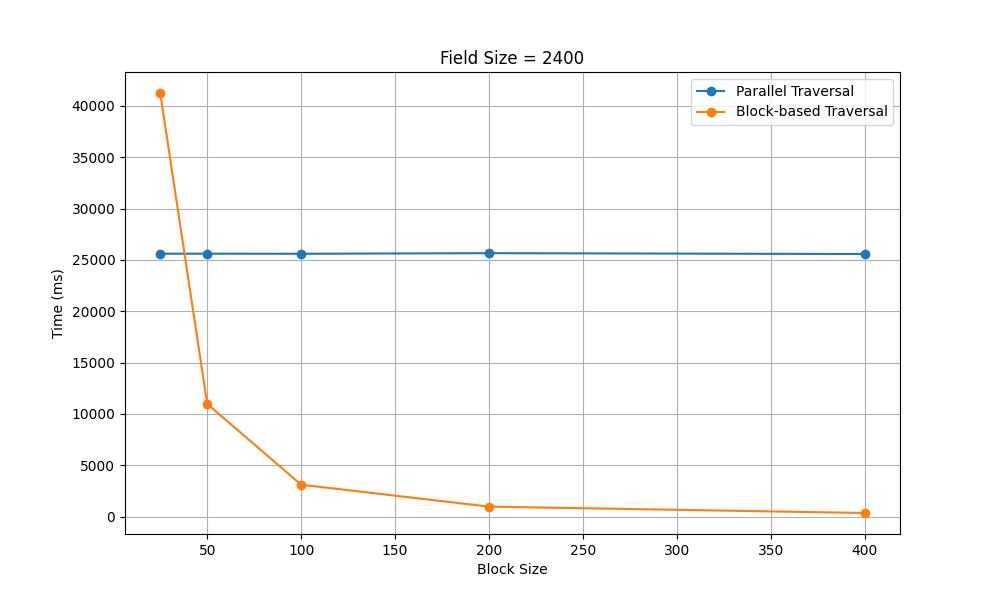
\includegraphics[width=\linewidth]{field_2400.png}
	\caption{The time of two kinds of Algorithms varies with Block Size}
\end{figure}

First, when we look at the time taken by the Parallel Traversal algorithm, it is clear that this value does not show any significant fluctuation when the block size changes, regardless of the field size. This is consistent with our understanding of the algorithm, as the Parallel Traversal does not incorporate the concept of block size in its design. Therefore, altering the block size does not directly affect its execution time.

Next, we turn our attention to the Block-based Traversal algorithm. From the data, we can see a clear trend of decreasing execution time as the block size increases. This is particularly evident when we compare the same field sizes. The reason behind this behavior is that the Block-based Traversal algorithm, by grouping the pixels into blocks, can reduce the number of checking operations when the block is completely inside or outside the polygon, thus enhancing the efficiency of rasterization. As the block size increases, the likelihood of this situation occurring is higher, hence the reduced execution time.

\begin{figure}[H] % Single column figure
	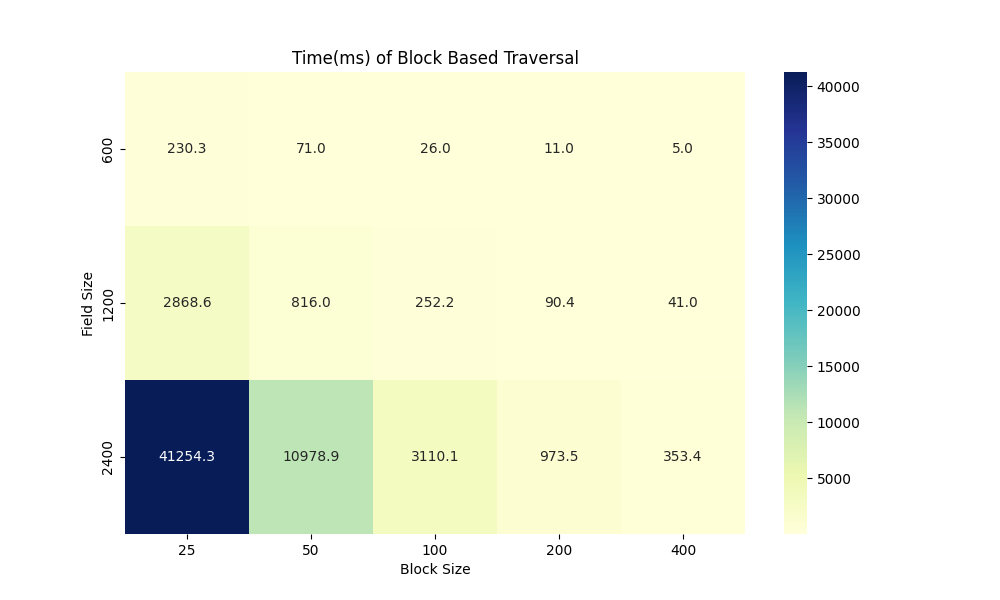
\includegraphics[width=\linewidth]{heat_map.png}
	\caption{The time(ms) of Block-based Traversal Algorithm}
\end{figure}

In summary, the Block-based Traversal algorithm shows clear advantages in efficiency over the Parallel Traversal algorithm, especially when the optimal block size is chosen for different field sizes. However, it is crucial to consider the trade-off between block size and field size in real-world applications to maximize performance.

%------------------------------------------------

\section{Conclusion}

Like Juan Pineda said:"There are many traversal algorithms possible. The best algorithm will depend on the cost/performance tradeoffs in the implementation."\cite{pineda1988} Although there are obvious advantages in time complexity using Block-based Traversal Algorithm, additional memory needs to be consumed to store mask information. Also the algorithm only simulate a simple rasterization which only judge whether pixels are in polygons. 

There are many more steps to rasterization, and this is only one of them; adapting Block-based Traversal algorithms to other steps such as anti-aliasing is a problem that will be considered in the future


%----------------------------------------------------------------------------------------
%	 REFERENCES
%----------------------------------------------------------------------------------------

\printbibliography

%----------------------------------------------------------------------------------------

\end{document}
